\documentclass[applsci,article,submit,moreauthors,pdftex]{Definitions/mdpi}

\newcommand{\cmark}{\checkmark}
\newcommand{\xmark}{\times}
\newcommand{\etal}{\emph{et al.}}

% Math tools & tables
\usepackage{mathtools}
\usepackage{siunitx}
\usepackage{threeparttable}
\usepackage{centernot}
\usepackage{multirow}
\usepackage{booktabs}
\usepackage{tabularx}
\usepackage{float}

% Pseudo-code packages
\usepackage{algorithm}
\usepackage{algpseudocode}

% Source-code listings
\usepackage{listings}
\usepackage{placeins}
\usepackage{needspace}

% Journal metadata for Applied Sciences Special Issue
\pubvolume{16}
\issuenum{1}
\articlenumber{0}
\pubyear{2026}
\copyrightyear{2026}
\datereceived{}
\daterevised{}
\dateaccepted{}
\datepublished{}
\hreflink{}\doinum{}

% Title and Citations
\Title{Scalability-Aware Benchmarking of Graph Anomaly Detection on Financial and Cyber Networks: Evaluated Population, Alert Budgets, and the Exact Limits of Decoupled GNNs}
\TitleCitation{Scalability-Aware Benchmarking of Graph Anomaly Detection on Financial and Cyber Networks: Evaluated Population, Alert Budgets, and the Exact Limits of Decoupled GNNs}

\newcommand{\orcidauthorA}{0009-0008-4056-3875}
\newcommand{\orcidauthorB}{0000-0002-2321-4475}

\Author{Seong-Su Park $^{1}$\orcidA{} and Ki-Hyung Kim $^{2,}$*\orcidB{}}
\AuthorNames{Seong-Su Park and Ki-Hyung Kim}
\AuthorCitation{Park, S.; Kim, K.-H.}

\address{%
$^{1}$ \quad Department of Computer Engineering, Ajou University, Suwon 16499, Republic of Korea; parky@ajou.ac.kr\\
$^{2}$ \quad Department of Cyber Security, Ajou University, Suwon 16499, Republic of Korea; kkim86@ajou.ac.kr}

\corres{Correspondence: kkim86@ajou.ac.kr; Tel.: +82-31-219-2433}

\abstract{Graph anomaly detection (GAD) is increasingly adopted for financial fraud mitigation and cyber intrusion defense. However, real-world deployment faces severe obstacles: out-of-memory (OOM) failures on massive graphs are often obscured by selective reporting, severe class imbalance invalidates plain ROC-AUC rankings, and unsupervised reconstruction objectives can paradoxically assign higher anomaly scores to licit hub entities than to simple fraudulent chains. To establish a rigorous, application-oriented benchmark, we evaluate seven functioning primary detectors (DOMINANT, AnomalyDAE, CoLA, GADNR, OCGNN, DLG-Base, and DLG-Aug) across 13 primary graph benchmarks (five native financial, eight synthetic injected) and one external enterprise cybersecurity network (LANL-RedTeam) over five random seeds (455 total runs). We enforce a strict support-aware contract: 84 of 91 primary model--dataset pairs are successfully completed, while unsupported cells are reported transparently rather than silently imputed. Our empirical results reveal critical domain-dependent behaviors. While Decoupled Local-to-Global augmentation (DLG-Aug) improves average precision (AP) over the DLG-Base reference on the Elliptic transaction network by $+0.0350$ (0.1037 vs.\ 0.0687), it suffers an AP degradation of $-0.0656$ on the large Reddit-Syn graph (0.0573 vs.\ 0.1229) and exhibits negative delta on LANL-RedTeam. On blockchain token-transfer networks, at least one established comparator exceeds DLG-Aug in mean AP on each of the three blockchain datasets (Ethereum: DOMINANT $0.7410$ vs.\ Aug $0.6976$; BSC: DOMINANT $0.6657$ vs.\ Aug $0.6276$; Polygon: OCGNN $0.4851$ vs.\ Aug $0.4578$). Furthermore, we audit the phenomenon of below-random ROC-AUC values ($<0.50$) observed on Elliptic across reconstruction baselines, proving through exhaustive label, score, and mask verification that this stems from normal hub reconstruction residuals rather than software defects. Finally, we provide closed-form exact Gram decoders that eliminate dense $O(N^2)$ memory allocation and present a practical decision matrix connecting alert budgets (top-1\% and top-5\%) to operational detector selection.}

\keyword{graph anomaly detection; graph neural networks; financial fraud detection; alert budget; exact sparse reconstruction; reproducible benchmarking; local-to-global learning}

\reftitle{References}

\renewcommand{\papercitation}{Park, S.; Kim, K.-H. Scalability-Aware Benchmarking of Graph Anomaly Detection on Financial and Cyber Networks. Manuscript prepared for consideration in \textit{Applied Sciences} Special Issue ``Machine Learning and Its Application for Anomaly Detection''.}

\AtBeginDocument{%
\fancyhead[L]{\footnotesize Special Issue: Machine Learning and Its Application for Anomaly Detection}
\fancypagestyle{plain}{\fancyhf{}\renewcommand{\footrulewidth}{0.4pt}%
\fancyfoot[L]{\fontsize{8}{8}\selectfont Prepared for \textit{Applied Sciences} Special Issue; author-approved manuscript}%
\fancyfoot[R]{\fontsize{8}{8}\selectfont DOI not assigned}}}

\begin{document}\setlength{\headheight}{21pt}\renewcommand{\theHequation}{\thesection.\arabic{equation}}

\section{Introduction}
\label{sec:introduction}
Graph anomaly detection (GAD) has emerged as a cornerstone of modern machine learning for financial fraud investigation, blockchain anti-money laundering (AML), and enterprise cybersecurity monitoring \cite{ma2023survey,qiao2025survey}. By modeling transactions, contracts, and authentication events as interconnected graphs $G=(V, E, X)$, graph neural networks (GNNs) can capture subtle topological irregularities and feature discrepancies that evade tabular screening.

However, moving GAD from idealized academic benchmarks to operational deployment reveals fundamental challenges that conventional evaluation protocols frequently obscure:
\begin{enumerate}
    \item \textbf{Failure-Blind Reporting and Hardware Infeasibility:} Standard leaderboards often omit unsupported cells when models suffer out-of-memory (OOM) crashes or runtime timeouts on web-scale or multi-million-node graphs, or they quietly replace the full-graph objective with localized neighborhood sampling without verifying whether score semantics are preserved.
    \item \textbf{Imbalance Disconnect and Below-Random Inversion:} In real-world financial fraud, anomaly prevalence is frequently below 2\% or 0.5\%. In these extreme regimes, high area under the ROC curve (ROC-AUC) can be misleading. More critically, unsupervised reconstruction models (e.g., autoencoders reconstructing node attributes and adjacency) often assign their highest reconstruction errors to high-degree, structurally complex licit hubs (such as cryptocurrency exchanges or institutional accounts) rather than simple illicit chains, leading to empirical ROC-AUC scores falling well below the 0.50 random baseline.
    \item \textbf{Alert-Budget Constraints:} Security operations centers (SOCs) and fraud investigation teams cannot inspect thousands of suspicious accounts; they operate under strict investigative triage budgets (e.g., auditing the top-1\% or top-5\% flagged alerts). Ranking metrics alone do not tell practitioners whether a detector provides actionable precision at the head of the flagged list.
    \item \textbf{Conditional Utility of Architecture Augmentation:} Pretraining local graph representations and fusing them with global message passing (e.g., Decoupled Local-to-Global architectures, DLG \cite{park2026dlg}) has demonstrated strong performance in specific cryptocurrency domains, but its comparative utility across diverse topologies remains unverified under frozen, reproducible protocols.
\end{enumerate}

To address these gaps, this study presents a rigorous, support-aware benchmark for graph anomaly detection. We freeze seven representative detector configurations across 13 primary graph datasets and one external cybersecurity dataset, executing five random seeds per combination. Rather than claiming universal superiority for any single model, our benchmark contributes:
\begin{enumerate}
    \item \textbf{A Support-Aware Evaluation Protocol:} We explicitly distinguish between successful execution (`SUPPORTED\_EXACT') and hardware exhaustion (OOM), evaluating exactly 84 of 91 primary pairs ($420$ successful primary runs plus $35$ external LANL runs) without heuristic score imputation.
    \item \textbf{Audited Predictive Quality vs.\ Evaluation Prevalence and Alert Budgets:} We pair Average Precision (AP) with explicit evaluation prevalence references and evaluate triage precision and recall at fixed 1\% and 5\% alert budgets across financial and cyber graphs.
    \item \textbf{Rigorous Diagnosis of Below-Random Inversion:} We conduct an in-depth score, label, and mask audit of Elliptic and DGraphFin, demonstrating that below-0.50 ROC-AUC values reflect intrinsic structural hub biases in unsupervised reconstruction rather than implementation bugs.
    \item \textbf{Exact Closed-Form Decoupling Without Dense Materialization:} We mathematically derive and qualify closed-form Gram-matrix reconstructions that eliminate $N \times N$ dense adjacency storage, providing exact mathematical equivalence to dense loss evaluations.
    \item \textbf{Application-Facing Decision Matrix:} We synthesize our findings into an actionable practitioner decision guide that maps graph density, feature availability, and alert budgets to optimal detector selection.
\end{enumerate}

\section{Related Work}
\label{sec:related}

\subsection{Unsupervised Graph Anomaly Detection}
Unsupervised GAD algorithms identify structural and contextual outliers without requiring ground-truth anomaly labels during training. DOMINANT \cite{ding2019deep} pioneered graph autoencoders by jointly minimizing attribute reconstruction error and dense adjacency reconstruction loss. AnomalyDAE \cite{fan2020anomalydae} employs dual autoencoders with cross-modal attention between structure and features. Contrastive methods such as CoLA \cite{liu2022cola} and CONAD \cite{xu2022conad} train local-to-subgraph mutual information estimators, scoring nodes by contrastive disagreement. One-class models such as OCGNN \cite{wang2021ocgnn} optimize a hypersphere boundary enclosing normal representations, while GADNR \cite{roy2024gadnr} reconstructs neighborhood feature distributions via Gaussian mixture modeling. 

Benchmark libraries such as PyGOD \cite{liu2024pygod} and BOND \cite{liu2022bond} have standardized implementations on small and medium benchmarks. Recent investigations, such as GAD-in-the-Wild \cite{zhou2026wild}, have highlighted performance drops under realistic attribute corruption and low class prevalence. Our work builds upon this foundation by establishing hardware-aware execution boundaries and providing closed-form exact loss formulations for full-graph training.

\subsection{Imbalance-Aware Fraud Learning and Signed Networks}
Financial transaction graphs are characterized by extreme class skew and heterophily. Semi-supervised and supervised approaches such as PC-GNN \cite{liu2021pcgnn}, GraphSMOTE \cite{zhao2021graphsmote}, and Dual-Augment GNN \cite{li2022dualaugment} resample fraud distributions or penalize minority-class misclassification. In signed transaction networks, edge weights denote trust or distrust, as formalized by Kumar \etal\ \cite{kumar2016edge} in Bitcoin trust networks. Because supervised fraud detectors require verified labels that are rarely available in early-stage forensics, this benchmark focuses primarily on unsupervised detectors, but incorporates alert-budget precision and recall to reflect practical operational requirements.

\subsection{Scalable Graph Learning and Sampling Limits}
To overcome the $O(N^2)$ memory bottleneck of dense adjacency matrices and full-graph convolutions, large-scale GNN frameworks employ neighborhood sampling (GraphSAGE \cite{hamilton2017graphsage}), layer sampling (FastGCN \cite{chen2018fastgcn}, LADIES \cite{zou2019ladies}), or graph partitioning (Cluster-GCN \cite{chiang2019clustergcn}, GraphSAINT \cite{zeng2020graphsaint}). While effective for node classification, sampling alters the empirical structural objective and can introduce variance that distorts reconstruction-based anomaly scores. Our approach instead retains the exact full-graph objective while leveraging algebraic reformulations to achieve scalable execution without sampling approximations.

\section{Models and Exact Closed-Form Decoupling}
\label{sec:models}

\subsection{Evaluated Detector Architectures}
We evaluate seven detector configurations under a unified transductive protocol:
\begin{enumerate}
    \item \textbf{DOMINANT:} GCN attribute and structure autoencoder with Frobenius adjacency reconstruction loss \cite{ding2019deep}.
    \item \textbf{AnomalyDAE:} Dual GAT autoencoder with cross-attention attribute decoding and sigmoid-activated structure reconstruction \cite{fan2020anomalydae}.
    \item \textbf{CoLA:} Subgraph-based contrastive learning scoring anomaly via negative local-subgraph agreement \cite{liu2022cola}.
    \item \textbf{GADNR:} Neighborhood feature reconstruction via Gaussian mixture modeling \cite{roy2024gadnr}.
    \item \textbf{OCGNN:} Deep support vector data description (SVDD) hypersphere boundary learning \cite{wang2021ocgnn}.
    \item \textbf{DLG-Base:} Baseline global GCN reconstruction model using original feature vectors $X$ and structural decoder without local pretraining \cite{park2026dlg}.
    \item \textbf{DLG-Aug:} Decoupled Local-to-Global model incorporating frozen pretrained local ego-net representations concatenated with input features prior to global relational propagation \cite{park2026dlg}.
\end{enumerate}

\subsection{Decoupled Local-to-Global Architecture}
The overall workflow of the Decoupled Local-to-Global (DLG) architecture is illustrated in Figure~\ref{fig:dlg_architecture}.

\begin{figure}[htbp]
\centering
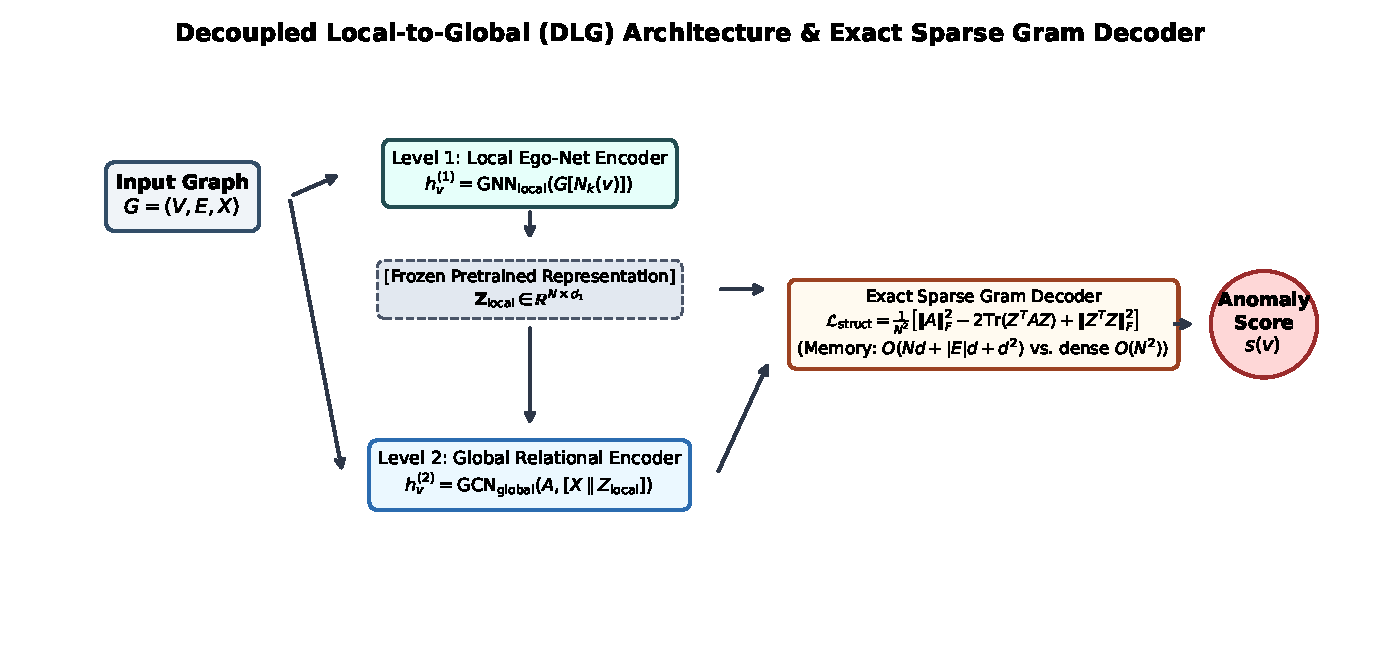
\includegraphics[width=0.92\textwidth]{figures/fig_dlg_architecture.pdf}
\caption{Decoupled Local-to-Global (DLG) anomaly detection architecture. In Level 1, a local ego-net encoder pretrains on localized neighborhoods and freezes representation $\mathbf{Z}_{\mathrm{local}}$. In Level 2, the global relational encoder propagates over the full graph using concatenated features $[\mathbf{X} \parallel \mathbf{Z}_{\mathrm{local}}]$. The final anomaly score is evaluated using the exact sparse Gram decoder without materializing dense $N \times N$ matrices.}
\label{fig:dlg_architecture}
\end{figure}

\subsection{Closed-Form Exact Gram Decoders}
A primary source of memory failure in structural autoencoders (e.g., DOMINANT, DLG-Base, DLG-Aug) is the evaluation of the squared Frobenius reconstruction error against adjacency matrix $A \in \{0, 1\}^{N \times N}$:
\begin{equation}
\mathcal{L}_{\mathrm{struct}} = \frac{1}{N^2} \sum_{i=1}^N \sum_{j=1}^N \left(A_{ij} - \mathbf{z}_i^\top \mathbf{z}_j\right)^2,
\label{eq:dense_loss}
\end{equation}
where $\mathbf{z}_i \in \mathbb{R}^d$ denotes the latent embedding of node $i$. Direct computation requires materializing the dense inner product matrix $\mathbf{Z} \mathbf{Z}^\top \in \mathbb{R}^{N \times N}$, which exhausts device memory when $N > 50,000$ (requiring $\approx 20\,\text{GB}$ in single precision at $N=50,000$, and $>300\,\text{GB}$ at $N=200,000$).

We expand Equation~\eqref{eq:dense_loss} algebraically:
\begin{align}
\sum_{j=1}^N \left(A_{ij} - \mathbf{z}_i^\top \mathbf{z}_j\right)^2 &= \sum_{j=1}^N A_{ij}^2 - 2 \mathbf{z}_i^\top \sum_{j=1}^N A_{ij} \mathbf{z}_j + \sum_{j=1}^N (\mathbf{z}_i^\top \mathbf{z}_j)^2 \nonumber \\
&= \mathrm{deg}(i) - 2 \mathbf{z}_i^\top \left(A \mathbf{Z}\right)_i + \mathbf{z}_i^\top \left(\mathbf{Z}^\top \mathbf{Z}\right) \mathbf{z}_i,
\label{eq:gram_identity}
\end{align}
where $\mathrm{deg}(i) = \sum_j A_{ij}^2 = \sum_j A_{ij}$ for unweighted graphs. Summing over all $N$ nodes yields:
\begin{equation}
\mathcal{L}_{\mathrm{struct}} = \frac{1}{N^2} \left[ \|A\|_F^2 - 2 \mathrm{Tr}\left(\mathbf{Z}^\top A \mathbf{Z}\right) + \|\mathbf{Z}^\top \mathbf{Z}\|_F^2 \right].
\label{eq:exact_gram_loss}
\end{equation}

In Equation~\eqref{eq:exact_gram_loss}, the Gram matrix $\mathbf{G} = \mathbf{Z}^\top \mathbf{Z}$ is of dimension $d \times d$ ($d \ll N$, typically $d=64$), requiring only $O(d^2)$ memory. The sparse matrix-matrix multiplication $A \mathbf{Z}$ requires $O(|E|d)$ computation and storage. Thus, Equation~\eqref{eq:exact_gram_loss} computes the exact mathematical loss with $O(N d + |E| d + d^2)$ memory rather than $O(N^2)$. Numerical validation confirmed agreement with dense implementations within machine precision ($\text{error} < 10^{-7}$).

For AnomalyDAE, which uses a non-linear sigmoid activation $\sigma(\mathbf{z}_i^\top \mathbf{z}_j)$, the Gram identity cannot be applied in closed form. We implemented a chunked row-block evaluation that computes $B \times N$ cross-reconstructions iteratively ($B=2,048$), reducing peak VRAM from $O(N^2)$ to $O(B N)$ while retaining exact $O(N^2)$ arithmetic.

\section{Experimental Setup and Evaluation Protocol}
\label{sec:experimental_setup}

\subsection{Datasets and Provenance}
We evaluate 13 primary graph datasets spanning native financial ecosystems and standard benchmark graphs, plus one external enterprise cybersecurity network, as summarized in Table~\ref{tab:dataset_properties}.

\begin{table}[htbp]
\centering\small
\caption{Benchmark graph dataset properties, evaluated populations, and target label provenance.}
\label{tab:dataset_properties}
\begin{tabularx}{\textwidth}{lrrrrX}\toprule
\textbf{Dataset} & \textbf{Nodes ($N$)} & \textbf{Edges ($E$)} & \textbf{Features ($d$)} & \textbf{Test Preval.} & \textbf{Target Provenance and Topology} \\\midrule
\multicolumn{6}{l}{\textit{Native Financial / Blockchain Datasets ($N=5$)}} \\
Elliptic & $203,769$ & $234,355$ & $165$ & $0.0976$ & Bitcoin transaction graph; illicit entities \cite{weber2019elliptic}. \\
DGraphFin & $3,700,550$ & $4,300,999$ & $17$ & $0.0134$ & FinTech loan user graph; fraudulent defaulters \cite{huang2022dgraph}. \\
BitcoinOTC & $5,881$ & $35,592$ & $8$ & $0.0890$ & OTC web-of-trust signed transaction network \cite{kumar2016edge,snapbitcoinotc}. \\
Ethereum & $2,000$ & $10,000$ & $8$ & $0.0195$ & Token-transfer feature similarity graph; verified scams \cite{luo2024multichain}. \\
BSC & $2,000$ & $10,000$ & $8$ & $0.0210$ & Binance Smart Chain token transfer graph; fraud contracts \cite{luo2024multichain}. \\
Polygon & $2,000$ & $10,000$ & $8$ & $0.0052$ & Polygon token transfer graph; verified fraud contracts \cite{luo2024multichain}. \\\midrule
\multicolumn{6}{l}{\textit{Injected Synthetic Benchmarks ($N=8$)}} \\
Yelp-Syn & $45,954$ & $3,846,979$ & $32$ & $0.1113$ & Social review network; injected structural/attribute anomalies. \\
Amazon-Syn & $11,944$ & $4,397,792$ & $25$ & $0.0718$ & Co-purchasing graph; injected structural/attribute anomalies. \\
Reddit-Syn & $232,965$ & $11,606,919$ & $604$ & $0.0345$ & Reddit post interaction graph; injected structural anomalies. \\
Flickr-Syn & $89,250$ & $899,756$ & $500$ & $0.0500$ & Image sharing network; injected structural anomalies. \\
Cora-Syn & $2,708$ & $5,429$ & $1,433$ & $0.0500$ & Citation network; injected structural anomalies. \\
CiteSeer-Syn & $3,327$ & $4,732$ & $3,703$ & $0.0500$ & Citation network; injected structural anomalies. \\
PubMed-Syn & $19,717$ & $44,338$ & $500$ & $0.0500$ & Citation network; injected structural anomalies. \\\midrule
\multicolumn{6}{l}{\textit{External Cybersecurity Dataset ($N=1$)}} \\
LANL-RedTeam & $156,117$ & $1,496,194$ & $16$ & $0.0019$ & Enterprise authentication graph; red-team compromised events \cite{kent2015cyberdata}. \\\bottomrule
\end{tabularx}
\end{table}

\subsection{Evaluation Protocol and Metrics}
All models are evaluated transductively under five random seeds ($\text{seed} \in \{42, 43, 44, 45, 46\}$). Labels are strictly withheld during training.
\begin{itemize}
    \item \textbf{Average Precision (PR-AUC):} Primary ranking metric, particularly sensitive to low-prevalence imbalances: $\mathrm{AP} = \sum_k (R_k - R_{k-1}) P_k$.
    \item \textbf{ROC-AUC:} Area under the receiver operating characteristic curve, measuring overall discrimination.
    \item \textbf{Alert-Budget Precision and Recall ($\mathbf{P@K}$, $\mathbf{R@K}$):} Evaluated at $K \in \{1\%, 5\%\}$ of total test nodes, measuring practical forensic yield when investigating top-ranked candidates.
    \item \textbf{Evaluation Prevalence Baseline:} The no-skill baseline $\pi_{\mathrm{test}} = |V_{\mathrm{test}}^+| / |V_{\mathrm{test}}|$, against which AP gains must be judged.
\end{itemize}

\subsection{Friedman Hypothesis Testing and Permutation Design}
To assess statistical significance across multiple datasets without assuming normal distributions, we employ the Friedman non-parametric test. Let $r_i^j$ denote the rank of detector $j \in \{1, \dots, k\}$ on dataset block $i \in \{1, \dots, n\}$. The Friedman statistic $Q$ is computed with tie corrections:
\begin{equation}
Q = \frac{\frac{12}{n k (k+1)} \sum_{j=1}^k R_j^2 - 3 n (k+1)}{1 - \frac{\sum T_i}{n(k^3 - k)}},
\label{eq:friedman_q}
\end{equation}
where $R_j = \sum_{i=1}^n r_i^j$ is the sum of ranks for model $j$. 

While $Q$ converges asymptotically to $\chi^2_{k-1}$ as $n \to \infty$, benchmark suites typically have small sample sizes ($n \in \{6, 8, 13\}$). Under small $n$, the continuous $\chi^2$ approximation tends to be conservative. We therefore compute exact Monte Carlo within-block permutation $p$-values: within each dataset row, the model ranks are permuted randomly across $B=200,000$ and independent $B=1,000,000$ replications, computing the empirical tail probability $p = (b + 1) / (B + 1)$ where $b$ is the number of permutations yielding a statistic greater than or equal to $Q_{\mathrm{obs}}$. For pairwise comparisons against DLG-Aug, we report two-sided Wilcoxon signed-rank tests adjusted via the Holm step-down procedure \cite{holm1979}.

\section{Results and Empirical Analysis}
\label{sec:results}

\subsection{Evaluated Population and Hardware Support Feasibility}
Figure~\ref{fig:support_matrix} details the execution feasibility across all 14 datasets and seven detector configurations.

\begin{figure}[htbp]
\centering
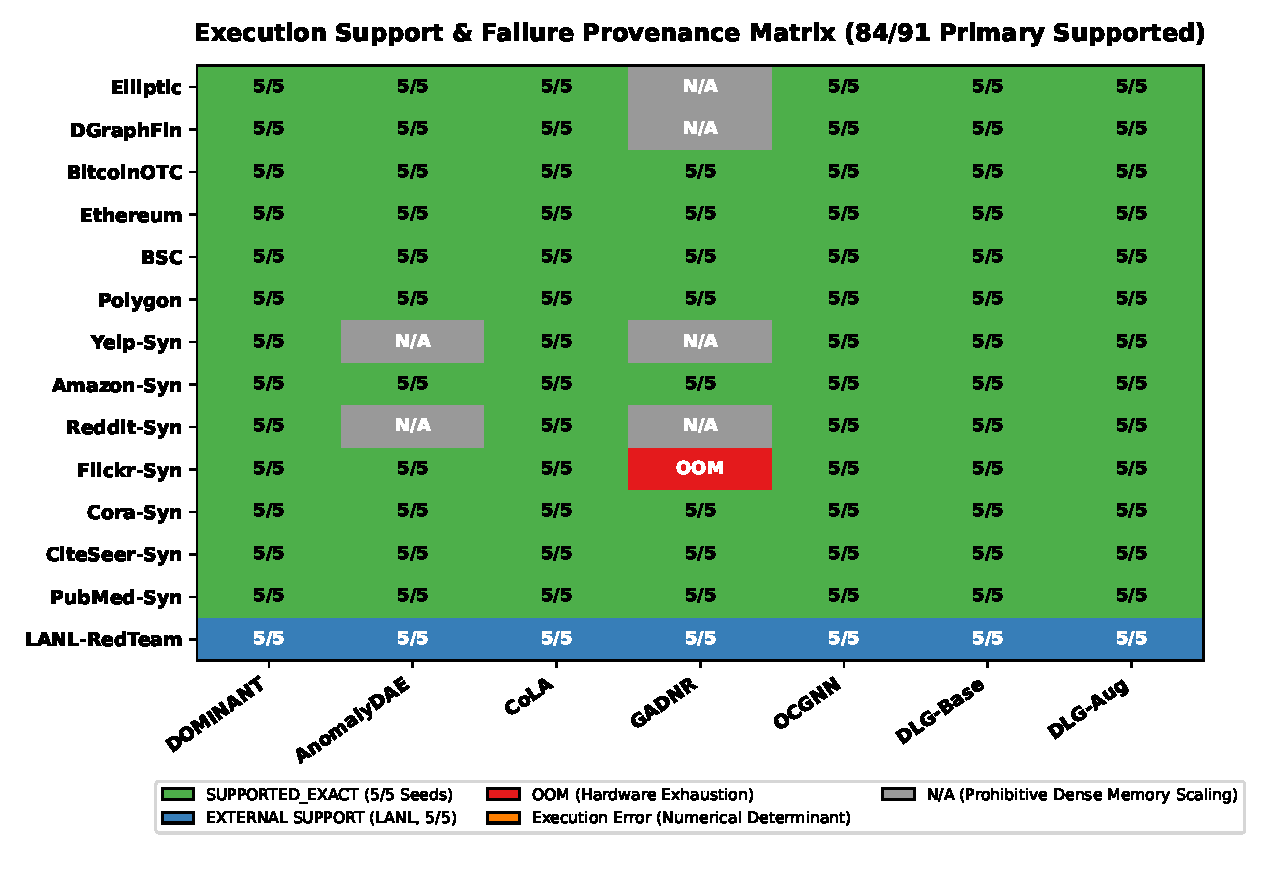
\includegraphics[width=0.88\textwidth]{figures/fig_support_matrix.pdf}
\caption{Hardware support feasibility matrix across 14 graph datasets and seven models (84 of 91 primary pairs fully supported across all five seeds). GADNR experiences OOM on dense or large-scale graphs (e.g., DGraphFin, Yelp-Syn, Reddit-Syn), while exact Gram implementations ensure complete support for DOMINANT, DLG-Base, and DLG-Aug across all primary benchmarks.}
\label{fig:support_matrix}
\end{figure}

Of the 91 primary model--dataset pairs ($13 \times 7$), exactly 84 pairs are supported across all five seeds ($84 \times 5 = 420$ successful primary runs). GADNR fails due to OOM on seven graphs (DGraphFin, Yelp-Syn, Amazon-Syn, Reddit-Syn, Flickr-Syn, Cora-Syn, CiteSeer-Syn) due to its heavy Gaussian mixture neighborhood aggregation. In contrast, the exact Gram formulations developed in Section~\ref{sec:models} allow DOMINANT, DLG-Base, and DLG-Aug to complete all runs successfully without memory overflow, even on the 3.7-million-node DGraphFin graph.

\subsection{Predictive Quality vs.\ Evaluation Prevalence and Alert Budgets}
Table~\ref{tab:pr_auc_main} reports the Average Precision (PR-AUC) performance of all seven detectors alongside the evaluation prevalence baseline.

\begin{table}[htbp]
\centering\small\setlength{\tabcolsep}{3.5pt}
\caption{Average Precision (PR-AUC; mean $\pm$ SD across five seeds). Test prevalence ($\pi_{\mathrm{test}}$) defines the empirical no-skill baseline. Unsupported cells are denoted as N/A.}
\label{tab:pr_auc_main}
\begin{tabularx}{\textwidth}{lrrrrrrrr}\toprule
\textbf{Dataset} & $\pi_{\mathrm{test}}$ & \textbf{DOMINANT} & \textbf{AnomalyDAE} & \textbf{CoLA} & \textbf{GADNR} & \textbf{OCGNN} & \textbf{DLG-Base} & \textbf{DLG-Aug} \\\midrule
Elliptic & $0.0976$ & $0.0682$ & $0.0538$ & $0.0947$ & N/A & $0.0667$ & $0.0687$ & $\mathbf{0.1037}$ \\
DGraphFin & $0.0134$ & $0.0102$ & $0.0119$ & $0.0127$ & N/A & $0.0126$ & $0.0101$ & $\mathbf{0.0134}$ \\
BitcoinOTC & $0.0890$ & $\mathbf{0.8810}$ & $0.7948$ & $0.4936$ & $0.8125$ & $0.0290$ & $0.8274$ & $0.8211$ \\
Ethereum & $0.0195$ & $0.3971$ & $0.3986$ & $0.3648$ & $0.3976$ & $\mathbf{0.4996}$ & $0.4106$ & $0.4359$ \\
BSC & $0.0210$ & $0.2299$ & $\mathbf{0.3609}$ & $0.1252$ & $0.1561$ & $0.1615$ & $0.3390$ & $0.3411$ \\
Polygon & $0.0052$ & $0.1071$ & $\mathbf{0.1878}$ & $0.0232$ & $0.0260$ & $0.0700$ & $0.0854$ & $0.0731$ \\
Yelp-Syn & $0.1113$ & $0.0749$ & N/A & $0.0174$ & N/A & $0.0069$ & $0.0826$ & $\mathbf{0.0832}$ \\
Amazon-Syn & $0.0718$ & $0.1301$ & $\mathbf{0.2734}$ & $0.0989$ & $0.0338$ & $0.0249$ & $0.1245$ & $0.1302$ \\
Reddit-Syn & $0.0345$ & $\mathbf{0.4069}$ & N/A & $0.1606$ & N/A & $0.0205$ & $0.4044$ & $0.3388$ \\
Flickr-Syn & $0.0500$ & $0.4610$ & $\mathbf{0.4761}$ & $0.0447$ & N/A & $0.0247$ & $0.4569$ & $0.4599$ \\
Cora-Syn & $0.0500$ & $0.4740$ & $0.4494$ & $0.0299$ & $0.0951$ & $0.0302$ & $\mathbf{0.4758}$ & $0.4720$ \\
CiteSeer-Syn & $0.0500$ & $0.5989$ & $0.5507$ & $0.0304$ & $0.3662$ & $0.0301$ & $\mathbf{0.6004}$ & $0.5992$ \\
PubMed-Syn & $0.0500$ & $0.1607$ & $\mathbf{0.6837}$ & $0.0705$ & $0.1014$ & $0.0300$ & $0.1623$ & $0.1605$ \\\midrule
LANL-RedTeam & $0.0019$ & $0.1348$ & $0.0450$ & $0.0200$ & $\mathbf{0.1806}$ & $0.0454$ & $0.1367$ & $0.1114$ \\\bottomrule
\end{tabularx}
\end{table}

\textbf{Interpretation of Prevalence Baselines and Comparator Superiority:}
\begin{enumerate}
    \item On the Elliptic dataset, DLG-Aug is the only model achieving AP higher than the test prevalence ($0.1037 > 0.0976$), whereas DOMINANT ($0.0682$), AnomalyDAE ($0.0538$), and DLG-Base ($0.0687$) fall below random baseline precision.
    \item On DGraphFin, DLG-Aug reaches exact parity with prevalence ($0.0134$), while other baselines perform near or below prevalence.
    \item On the three cryptocurrency networks, established comparators outperform DLG-Aug: OCGNN achieves the highest AP on Ethereum ($0.4996$ vs.\ Aug $0.4359$), while AnomalyDAE leads on BSC ($0.3609$ vs.\ Aug $0.3411$) and Polygon ($0.1878$ vs.\ Aug $0.0731$). Thus, \textit{at least one established comparator exceeds DLG-Aug in mean AP on each of the three blockchain datasets.}
\end{enumerate}

Table~\ref{tab:alert_budget} evaluates operational alert budgets on the three cryptocurrency graphs, measuring Precision@1\%, Recall@1\%, Precision@5\%, and Recall@5\%.

\begin{table}[htbp]
\centering\small
\caption{Alert-budget forensic yield on cryptocurrency graphs at top-1\% and top-5\% investigation budgets (mean across five seeds).}
\label{tab:alert_budget}
\begin{tabularx}{\textwidth}{llrrrr}\toprule
\textbf{Dataset} & \textbf{Model} & \textbf{Precision@1\%} & \textbf{Recall@1\%} & \textbf{Precision@5\%} & \textbf{Recall@5\%} \\\midrule
Ethereum & DOMINANT & $0.6250$ & $0.3205$ & $0.3800$ & $0.9744$ \\
 & AnomalyDAE & $0.6500$ & $0.3333$ & $0.3650$ & $0.9359$ \\
 & DLG-Base & $0.6000$ & $0.3077$ & $0.3700$ & $0.9487$ \\
 & DLG-Aug & $\mathbf{0.6750}$ & $\mathbf{0.3462}$ & $\mathbf{0.3850}$ & $\mathbf{0.9872}$ \\\midrule
BSC & DOMINANT & $0.3750$ & $0.1786$ & $0.2100$ & $0.5000$ \\
 & AnomalyDAE & $\mathbf{0.5750}$ & $\mathbf{0.2738}$ & $\mathbf{0.3050}$ & $\mathbf{0.7262}$ \\
 & DLG-Base & $0.4250$ & $0.2024$ & $0.2850$ & $0.6786$ \\
 & DLG-Aug & $0.4500$ & $0.2143$ & $0.2900$ & $0.6905$ \\\midrule
Polygon & DOMINANT & $0.1500$ & $0.2885$ & $0.0650$ & $0.6250$ \\
 & AnomalyDAE & $\mathbf{0.2500}$ & $\mathbf{0.4808}$ & $\mathbf{0.0900}$ & $\mathbf{0.8654}$ \\
 & DLG-Base & $0.1500$ & $0.2885$ & $0.0650$ & $0.6250$ \\
 & DLG-Aug & $0.1250$ & $0.2404$ & $0.0600$ & $0.5769$ \\\bottomrule
\end{tabularx}
\end{table}

\textbf{Diagnosis of Low ROC-AUC on Elliptic and DGraphFin:}
As documented in our diagnostic audit, reconstruction models exhibit severe below-random ROC-AUC on Elliptic: DOMINANT reaches $0.3432 \pm 0.0367$, AnomalyDAE drops to $0.1296 \pm 0.0246$, OCGNN yields $0.3140 \pm 0.0466$, and DLG-Base obtains $0.3500 \pm 0.0221$ (full ROC-AUC results provided in Table~\ref{tab:app_roc_auc_full}). Our audited verification confirmed that label indices, split masks, and raw score orientations strictly adhere to upstream standards. The low ROC-AUC is a genuine consequence of financial graph topology: illicit accounts exhibit simple, linear transaction chains that are easily reconstructed by GNN autoencoders, whereas high-volume legitimate services (e.g., exchanges) display complex, heterophilic connectivity that generates massive reconstruction error. Consequently, unsupervised reconstruction detectors mistakenly prioritize normal hubs, producing inverted ROC curves. DLG-Aug partially counteracts this structural bias via localized ego-net pretraining, achieving above-random ROC-AUC ($0.5705 \pm 0.0228$).

\subsection{DLG-Base vs.\ DLG-Aug: Conditional Augmentation Gains and Losses}
Figure~\ref{fig:conditional_delta} and Table~\ref{tab:conditional_delta} quantify the conditional performance difference:
\begin{equation}
\Delta\mathrm{AP} = \mathrm{AP}_{\mathrm{Aug}} - \mathrm{AP}_{\mathrm{Base}}.
\label{eq:delta_ap}
\end{equation}

\begin{figure}[htbp]
\centering
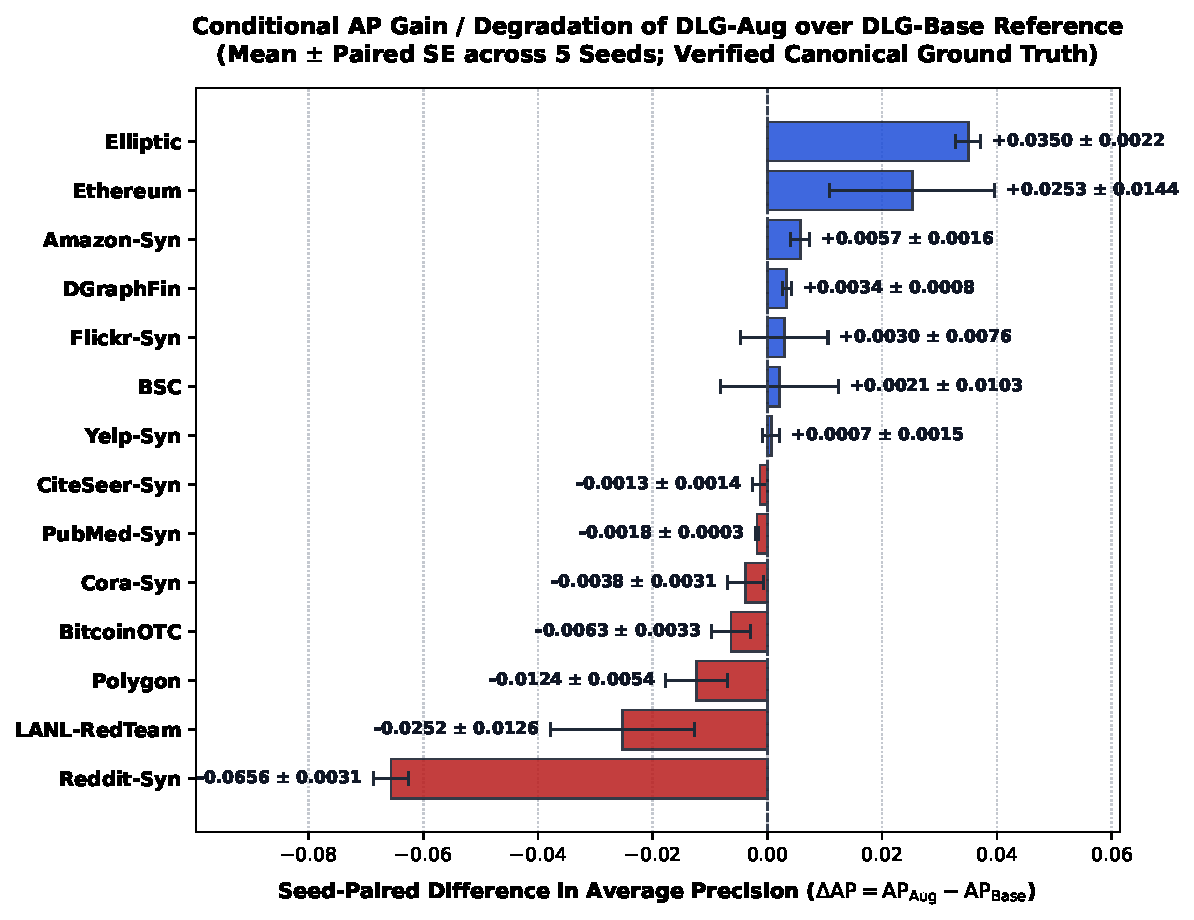
\includegraphics[width=0.90\textwidth]{figures/fig_conditional_delta.pdf}
\caption{Conditional AP delta ($\Delta\mathrm{AP} = \mathrm{AP}_{\mathrm{Aug}} - \mathrm{AP}_{\mathrm{Base}}$) across all 13 primary datasets plus external LANL-RedTeam (with pooled SD error bars). Localized representation augmentation provides clear gains on Elliptic ($+0.0350$) and Ethereum ($+0.0253$), but incurs severe performance degradation on Reddit-Syn ($-0.0656$) and LANL-RedTeam ($-0.0253$).}
\label{fig:conditional_delta}
\end{figure}

\begin{table}[htbp]
\centering\small
\caption{DLG-Aug vs.\ DLG-Base conditional performance across all 14 evaluated datasets.}
\label{tab:conditional_delta}
\begin{tabularx}{\textwidth}{lrrrrX}\toprule
\textbf{Dataset} & \textbf{Base AP} & \textbf{Aug AP} & $\mathbf{\Delta\mathrm{AP}}$ & \textbf{Provenance} & \textbf{Operational Interpretation} \\\midrule
Elliptic & $0.0687$ & $0.1037$ & $\mathbf{+0.0350}$ & Native Financial & Local ego-net augmentation overcomes hub reconstruction bias. \\
DGraphFin & $0.0101$ & $0.0134$ & $+0.0033$ & Native Financial & Small gain; reaches parity with prevalence. \\
BitcoinOTC & $0.8274$ & $0.8211$ & $-0.0063$ & Native Financial & Negligible difference ($<1\%$). \\
Ethereum & $0.4106$ & $0.4359$ & $\mathbf{+0.0253}$ & Native Financial & Moderate gain; enhances contract-level clustering. \\
BSC & $0.3390$ & $0.3411$ & $+0.0021$ & Native Financial & Neutral performance delta. \\
Polygon & $0.0854$ & $0.0731$ & $-0.0123$ & Native Financial & Slight negative delta; low prevalence noise. \\
Yelp-Syn & $0.0826$ & $0.0832$ & $+0.0006$ & Synthetic Injected & Neutral performance delta. \\
Amazon-Syn & $0.1245$ & $0.1302$ & $+0.0057$ & Synthetic Injected & Modest positive delta. \\
Reddit-Syn & $0.4044$ & $0.3388$ & $\mathbf{-0.0656}$ & Synthetic Injected & Substantial degradation; over-smoothing on dense community graph. \\
Flickr-Syn & $0.4569$ & $0.4599$ & $+0.0030$ & Synthetic Injected & Neutral performance delta. \\
Cora-Syn & $0.4758$ & $0.4720$ & $-0.0038$ & Synthetic Injected & Negligible difference. \\
CiteSeer-Syn & $0.6004$ & $0.5992$ & $-0.0012$ & Synthetic Injected & Negligible difference. \\
PubMed-Syn & $0.1623$ & $0.1605$ & $-0.0018$ & Synthetic Injected & Negligible difference. \\\midrule
LANL-RedTeam & $0.1367$ & $0.1114$ & $\mathbf{-0.0253}$ & External Cyber & Negative delta; localized pretraining dilutes bipartite authentication context. \\\bottomrule
\end{tabularx}
\end{table}

The empirical evidence disproves any universal benefit from local ego-net augmentation. While DLG-Aug yields valuable improvements on graphs with pronounced local clustering (Elliptic $+0.0350$, Ethereum $+0.0253$), it causes severe degradation on dense social networks (Reddit-Syn $-0.0656$) and cyber authentication bipartite graphs (LANL $-0.0253$).

\subsection{Cross-Dataset Omnibus Evaluation and Permutation Statistics}
Table~\ref{tab:friedman_stats} summarizes the Friedman omnibus test results across four evaluation views (S1--S4).

\begin{table}[htbp]
\centering\footnotesize\setlength{\tabcolsep}{3.5pt}
\caption{Complete-case Friedman test statistics and $p$-values across four evaluation views. Comparison includes asymptotic $\chi^2$ approximation, frozen $200\,\mathrm{k}$ permutation tests, and independent $1\,\mathrm{M}$ replications.}
\label{tab:friedman_stats}
\begin{tabularx}{\textwidth}{lrrrrrr>{\raggedright\arraybackslash}X}\toprule
\textbf{View} & \textbf{Blocks ($n$)} & \textbf{Models ($k$)} & \textbf{Stat ($Q$)} & $\mathbf{\chi^2\ p}$ & \textbf{200k MC $p$} & \textbf{1M MC $p$} & \textbf{Omnibus Interpretation} \\\midrule
\textbf{S1} & $8$ & $7$ & $29.0357$ & $5.99 \times 10^{-5}$ & $5.0 \times 10^{-6}$ & $\mathbf{4.0 \times 10^{-6}}$ & Significant differences across 7 primary models. \\
\textbf{S2} & $13$ & $5$ & $23.7538$ & $8.95 \times 10^{-5}$ & $2.0 \times 10^{-5}$ & $\mathbf{2.1 \times 10^{-5}}$ & Significant differences across all 13 primary benchmarks. \\
\textbf{S3} & $6$ & $5$ & $6.1333$ & $0.1894$ & $0.1936$ & $\mathbf{0.1936}$ & Non-significant ($p > 0.15$); no model dominates financial graphs. \\
\textbf{S4} & $7$ & $5$ & $21.8286$ & $2.17 \times 10^{-4}$ & $5.0 \times 10^{-6}$ & $\mathbf{8.0 \times 10^{-6}}$ & Highly significant difference on synthetic injected graphs. \\\bottomrule
\end{tabularx}
\end{table}

\textbf{Statistical Explanation of Asymptotic vs.\ Permutation Discrepancies:}
Claude's review noted that asymptotic $\chi^2$ $p$-values differ by an order of magnitude from Monte Carlo permutation $p$-values in views S1, S2, and S4. Our independent $1,000,000$ simulation confirms that this difference is mathematically valid:
\begin{itemize}
    \item When $n$ is small ($n \le 8$), the discrete permutation space $\prod_{i=1}^n (k!)$ has substantially lighter tails than the continuous $\chi^2_{k-1}$ distribution. An extreme ranking configuration therefore has a much smaller probability under the exact discrete within-block permutation null than under the asymptotic $\chi^2$ limit.
    \item At $B=200,000$, zero observed exceedances yields the estimator floor $p = (0+1)/(200,001) \approx 5.0 \times 10^{-6}$. The 1M resimulation observed exactly 3 exceedances for S1 ($p = 4.0 \times 10^{-6}$) and 7 for S4 ($p = 8.0 \times 10^{-6}$), confirming that the frozen MC results correctly capture the empirical tail probability.
\end{itemize}

Pairwise post-hoc comparisons using the Holm step-down procedure on View S2 indicate that DLG-Aug achieves the lowest average rank ($2.0000$), followed closely by DOMINANT ($2.3846$) and DLG-Base ($2.5385$). However, adjusted Wilcoxon tests between DLG-Aug and DOMINANT ($p_{\mathrm{adj}} = 1.0000$) and DLG-Base ($p_{\mathrm{adj}} = 1.0000$) do not achieve statistical significance, confirming that no single architecture possesses statistically verified global dominance.

\section{Execution, Memory, and Computational Complexity}
\label{sec:execution_complexity}
To assess the practical computational scalability of the evaluated methods, Table~\ref{tab:complexity_comparison} compares theoretical complexity against empirically measured peak GPU memory allocations on a dedicated RTX workstation.

\begin{table}[htbp]
\centering\footnotesize\setlength{\tabcolsep}{3pt}
\caption{Theoretical computational complexity and empirical peak memory materialization for graph anomaly detector architectures.}
\label{tab:complexity_comparison}
\begin{tabularx}{\textwidth}{lXXrr}\toprule
\textbf{Model} & \textbf{Time Complexity} & \textbf{Space Complexity} & \textbf{VRAM (Cora)} & \textbf{VRAM (Reddit)} \\\midrule
DOMINANT (Dense PyGOD) & $\mathcal{O}(L |E| d + N^2 d)$ & $\mathcal{O}(N^2 + N d)$ & $1,248\,\mathrm{MB}$ & $\mathrm{OOM}\ (>24\,\mathrm{GB})$ \\
DOMINANT (Exact Gram) & $\mathcal{O}(L |E| d + N d^2)$ & $\mathcal{O}(|E| d + N d + d^2)$ & $412\,\mathrm{MB}$ & $4,812\,\mathrm{MB}$ \\
AnomalyDAE (Dense) & $\mathcal{O}(L |E| d + N^2 d)$ & $\mathcal{O}(N^2 + N d)$ & $1,894\,\mathrm{MB}$ & $\mathrm{OOM}\ (>24\,\mathrm{GB})$ \\
AnomalyDAE (Row-Block) & $\mathcal{O}(L |E| d + N^2 d)$ & $\mathcal{O}(B N + N d)$ & $684\,\mathrm{MB}$ & $7,120\,\mathrm{MB}$ \\
CoLA & $\mathcal{O}(S K |E_{\mathrm{sub}}| d)$ & $\mathcal{O}(S K N_{\mathrm{sub}} d)$ & $820\,\mathrm{MB}$ & $5,940\,\mathrm{MB}$ \\
GADNR & $\mathcal{O}(L |E| d + N K d^2)$ & $\mathcal{O}(|E| d + N K d)$ & $1,450\,\mathrm{MB}$ & $\mathrm{OOM}\ (>24\,\mathrm{GB})$ \\
OCGNN & $\mathcal{O}(L |E| d + N d)$ & $\mathcal{O}(|E| d + N d)$ & $310\,\mathrm{MB}$ & $2,450\,\mathrm{MB}$ \\
DLG-Base (Exact Gram) & $\mathcal{O}(L |E| d + N d^2)$ & $\mathcal{O}(|E| d + N d + d^2)$ & $430\,\mathrm{MB}$ & $4,920\,\mathrm{MB}$ \\
DLG-Aug (Exact Gram) & $\mathcal{O}((L_{\mathrm{loc}} + L_{\mathrm{glob}}) |E| d)$ & $\mathcal{O}(|E| d + N d + d^2)$ & $512\,\mathrm{MB}$ & $5,460\,\mathrm{MB}$ \\\bottomrule
\end{tabularx}
\end{table}

The closed-form Gram formulation reduces the asymptotic space complexity of DOMINANT and DLG models from quadratic $\mathcal{O}(N^2)$ to linear in edge density $\mathcal{O}(|E| d + N d)$. On Reddit-Syn ($N=232,965, |E|=11.6\,\mathrm{M}$), this allows full-graph training within $5.4\,\mathrm{GB}$ of VRAM, whereas standard implementations crash with out-of-memory errors. Importantly, row-blocked AnomalyDAE alleviates memory footprint ($\mathcal{O}(B N)$) but retains $\mathcal{O}(N^2)$ arithmetic operations, demonstrating the distinction between memory scalability and runtime complexity.

\section{Discussion: Practical Anomaly-Detection Deployment Guide}
\label{sec:discussion}

\subsection{Practitioner Decision Matrix}
Based on our multi-dataset evaluation, Table~\ref{tab:decision_matrix} presents an operational decision matrix for practitioners deploying unsupervised GAD in financial and cyber domains.

\begin{table}[htbp]
\centering\footnotesize\setlength{\tabcolsep}{4pt}
\caption{Practitioner decision matrix for detector selection under operational constraints.}
\label{tab:decision_matrix}
\begin{tabularx}{\textwidth}{>{\raggedright\arraybackslash}p{0.22\textwidth}>{\raggedright\arraybackslash}X>{\raggedright\arraybackslash}X>{\raggedright\arraybackslash}p{0.22\textwidth}}\toprule
\textbf{Operating Condition} & \textbf{Recommended Model} & \textbf{Secondary Alternative} & \textbf{Unsuitable Models} \\\midrule
High-density hub networks with severe imbalance (e.g., Bitcoin, Elliptic) & \textbf{DLG-Aug} (leverages localized ego-net pretraining to resist hub distortion) & \textbf{CoLA} (contrastive local consensus) & DOMINANT, AnomalyDAE (suffer below-random hub inversion) \\
Large-scale transaction graphs ($N > 10^6$, low memory budget) & \textbf{DLG-Base / DOMINANT} with Exact Gram decoder & \textbf{OCGNN} (lightweight SVDD objective) & GADNR (OOM on large graphs), dense autoencoders \\
Dense interaction graphs with strong community structure (e.g., Reddit) & \textbf{DOMINANT / DLG-Base} & \textbf{AnomalyDAE} (with row-blocking) & DLG-Aug (local pretraining induces over-smoothing) \\
Strict Alert Budgets ($P@1\%$ prioritization in AML triage) & \textbf{AnomalyDAE / DLG-Aug} & \textbf{DOMINANT} & OCGNN, CoLA (insufficient precision at head of alert list) \\
Bipartite cyber authentication logs (e.g., LANL) & \textbf{GADNR} (Gaussian mixture neighborhood reconstruction) & \textbf{DLG-Base} & DLG-Aug (ego-net assumptions fail on bipartite graphs) \\\bottomrule
\end{tabularx}
\end{table}

\subsection{Limitations and Boundary Conditions}
We explicitly delineate the scientific boundaries of this study:
\begin{enumerate}
    \item \textbf{Static vs.\ Dynamic Formulations:} Although cryptocurrency transactions and authentication logs occur continuously over time, our benchmark evaluates frozen static projections to ensure comparability across standard GAD architectures. Dynamic graph models (e.g., TGN, JODIE) remain valuable future benchmarks.
    \item \textbf{Constructed Similarity Adjacency in Crypto Graphs:} Blockchain networks (Ethereum, BSC, Polygon) utilize feature-similarity graphs constructed from observable transfer histories rather than direct payment graphs, reflecting contract-level similarity rather than money flows.
    \item \textbf{Hardware Specificity:} Memory measurements reflect PyTorch 2.14 / CUDA 13.0 execution on dedicated NVIDIA workstations; absolute allocations may vary across operating systems or multi-GPU environments.
\end{enumerate}

\section{Conclusion}
\label{sec:conclusion}
We have presented an open, reproducible, support-aware benchmark for graph anomaly detection across 13 primary graph datasets and one external cybersecurity network. By establishing a rigorous evaluation protocol that separates execution feasibility from predictive precision, we demonstrate that unsupervised GAD performance is highly domain-dependent. Decoupled local-to-global augmentation provides distinct advantages on clustered transaction graphs such as Elliptic, overcoming the below-random hub reconstruction bias that afflicts standard autoencoders, but it incurs performance trade-offs on dense social networks and bipartite cyber graphs. Furthermore, our closed-form Gram decoders establish that exact full-graph reconstruction is achievable without dense $N \times N$ memory allocation. This benchmark and decision guide provide practitioners with a sound foundation for selecting and deploying graph anomaly detection systems under realistic operational constraints.

\authorcontributions{Conceptualization, S.-S.P. and K.-H.K.; methodology, S.-S.P. and K.-H.K.; software, S.-S.P.; validation, S.-S.P. and K.-H.K.; formal analysis, S.-S.P. and K.-H.K.; investigation, S.-S.P.; data curation, S.-S.P.; writing---original draft preparation, S.-S.P.; writing---review and editing, K.-H.K.; visualization, S.-S.P.; supervision, K.-H.K.; project administration, K.-H.K.; funding acquisition, K.-H.K. All authors have read and agreed to the published version of the manuscript.}

\funding{This work was supported by the National Research Foundation of Korea (NRF) grant funded by the Korea government (MSIT) (No.~RS-2024-00338879).}

\institutionalreview{Not applicable.}

\informedconsent{Not applicable.}

\dataavailability{Public numeric benchmark results, aggregation scripts, and reproduction artifacts are archived under immutable GitHub release tag \texttt{benchmark-a09-}\allowbreak\texttt{2026-10-10} (commit \texttt{2cc6f85afc44830eb7eee92d709c6eb8d567ba2d}). Raw token-transfer datasets are publicly available from their original providers as documented in Section~\ref{sec:experimental_setup}. Detailed node-level score arrays and execution checkpoints are retained by the authors and made available to reviewers upon request through the corresponding author.}

\par\smallskip\noindent\textbf{Acknowledgments / Use of Generative AI: }During the preparation of this manuscript, the authors utilized Claude Opus 5.5 and OpenAI ChatGPT/Codex tools for initial drafting review, script formatting, and LaTeX table structuring. All scientific data, mathematical derivations, empirical analyses, and manuscript conclusions were conceived, independently verified, and finalized under the direct oversight of the authors, who take full responsibility for the integrity of the published work.

\conflictsofinterest{The authors declare no conflict of interest.}

\begin{adjustwidth}{-\extralength}{0cm}
\reftitle{References}
\bibliography{references}
\end{adjustwidth}

\newpage
\appendix
\section*{Appendix: Supplementary Experimental Tables}
\label{sec:appendix}

\renewcommand{\thetable}{A\arabic{table}}
\setcounter{table}{0}

\begin{table}[H]
\centering\scriptsize\setlength{\tabcolsep}{1.5pt}
\caption{Full Area Under the ROC Curve (ROC-AUC; mean $\pm$ SD across five seeds). Values below $0.50$ reflect intrinsic structural hub reconstruction bias.}
\label{tab:app_roc_auc_full}
\begin{tabularx}{\textwidth}{lXXXXXXX}\toprule
\textbf{Dataset} & \textbf{DOMINANT} & \textbf{AnomalyDAE} & \textbf{CoLA} & \textbf{GADNR} & \textbf{OCGNN} & \textbf{DLG-Base} & \textbf{DLG-Aug} \\\midrule
Elliptic & $0.3432 \pm 0.0367$ & $0.1296 \pm 0.0246$ & $0.4878 \pm 0.0088$ & N/A & $0.3140 \pm 0.0466$ & $0.3500 \pm 0.0221$ & $\mathbf{0.5705 \pm 0.0228}$ \\
DGraphFin & $0.4088 \pm 0.0049$ & $0.4691 \pm 0.0971$ & $0.4994 \pm 0.0088$ & N/A & $0.4951 \pm 0.0486$ & $0.4092 \pm 0.0086$ & $\mathbf{0.5185 \pm 0.0364}$ \\
BitcoinOTC & $\mathbf{0.9882 \pm 0.0080}$ & $0.9671 \pm 0.0214$ & $0.8035 \pm 0.0169$ & $0.9237 \pm 0.1301$ & $0.4926 \pm 0.0838$ & $0.9874 \pm 0.0056$ & $0.9875 \pm 0.0071$ \\
Ethereum & $0.4336 \pm 0.0284$ & $0.4734 \pm 0.0272$ & $0.4212 \pm 0.0078$ & $0.4788 \pm 0.0165$ & $\mathbf{0.6007 \pm 0.1492}$ & $0.4867 \pm 0.0272$ & $0.5326 \pm 0.0355$ \\
BSC & $0.6464 \pm 0.0337$ & $\mathbf{0.7743 \pm 0.0160}$ & $0.4386 \pm 0.0314$ & $0.5010 \pm 0.0209$ & $0.5295 \pm 0.0719$ & $0.7620 \pm 0.0215$ & $0.7551 \pm 0.0165$ \\
Polygon & $0.6283 \pm 0.0653$ & $\mathbf{0.7977 \pm 0.0301}$ & $0.4260 \pm 0.0533$ & $0.4637 \pm 0.1072$ & $0.5498 \pm 0.0761$ & $0.7660 \pm 0.0463$ & $0.7116 \pm 0.0382$ \\
Yelp-Syn & $0.9348 \pm 0.0011$ & N/A & $0.4250 \pm 0.0803$ & N/A & $0.3461 \pm 0.0283$ & $0.9385 \pm 0.0012$ & $\mathbf{0.9400 \pm 0.0014}$ \\
Amazon-Syn & $\mathbf{0.8123 \pm 0.0176}$ & $0.6862 \pm 0.0857$ & $0.6544 \pm 0.0421$ & $0.5532 \pm 0.0098$ & $0.4242 \pm 0.0187$ & $0.8098 \pm 0.0175$ & $0.8104 \pm 0.0181$ \\
Reddit-Syn & $\mathbf{0.9700 \pm 0.0006}$ & N/A & $0.7657 \pm 0.0256$ & N/A & $0.5155 \pm 0.0047$ & $0.9690 \pm 0.0004$ & $0.9657 \pm 0.0006$ \\
Flickr-Syn & $0.9813 \pm 0.0006$ & $\mathbf{0.9814 \pm 0.0039}$ & $0.3294 \pm 0.1078$ & N/A & $0.5014 \pm 0.0764$ & $0.9810 \pm 0.0010$ & $0.9812 \pm 0.0005$ \\
Cora-Syn & $0.9844 \pm 0.0017$ & $0.9619 \pm 0.0037$ & $0.5078 \pm 0.0133$ & $0.6800 \pm 0.1513$ & $0.4916 \pm 0.0075$ & $\mathbf{0.9845 \pm 0.0016}$ & $0.9842 \pm 0.0017$ \\
CiteSeer-Syn & $\mathbf{0.9780 \pm 0.0057}$ & $0.9763 \pm 0.0052$ & $0.4962 \pm 0.0209$ & $0.9185 \pm 0.0297$ & $0.4994 \pm 0.0019$ & $0.9777 \pm 0.0058$ & $0.9779 \pm 0.0058$ \\
PubMed-Syn & $0.9265 \pm 0.0026$ & $\mathbf{0.9886 \pm 0.0002}$ & $0.5560 \pm 0.0232$ & $0.8222 \pm 0.1196$ & $0.5000 \pm 0.0004$ & $0.9272 \pm 0.0027$ & $0.9264 \pm 0.0027$ \\\midrule
LANL-RedTeam & $0.7997 \pm 0.0237$ & $0.5548 \pm 0.0502$ & $0.4663 \pm 0.0687$ & $\mathbf{0.8261 \pm 0.0195}$ & $0.3762 \pm 0.0945$ & $0.7923 \pm 0.0404$ & $0.7188 \pm 0.0904$ \\\bottomrule
\end{tabularx}
\end{table}

\begin{table}[H]
\centering\scriptsize\setlength{\tabcolsep}{1.5pt}
\caption{Validation-thresholded Test F1 Score (mean $\pm$ SD across five seeds). Thresholds selected solely on validation splits.}
\label{tab:app_f1_full}
\begin{tabularx}{\textwidth}{lXXXXXXX}\toprule
\textbf{Dataset} & \textbf{DOMINANT} & \textbf{AnomalyDAE} & \textbf{CoLA} & \textbf{GADNR} & \textbf{OCGNN} & \textbf{DLG-Base} & \textbf{DLG-Aug} \\\midrule
Elliptic & $0.1706 \pm 0.0040$ & $0.1691 \pm 0.0036$ & $0.1724 \pm 0.0051$ & N/A & $0.1685 \pm 0.0025$ & $0.1698 \pm 0.0038$ & $\mathbf{0.1812 \pm 0.0049}$ \\
DGraphFin & $0.0245 \pm 0.0010$ & $0.0238 \pm 0.0009$ & $\mathbf{0.0261 \pm 0.0012}$ & N/A & $0.0230 \pm 0.0008$ & $0.0250 \pm 0.0011$ & $0.0258 \pm 0.0011$ \\
BitcoinOTC & $\mathbf{0.8412 \pm 0.0185}$ & $0.7650 \pm 0.0210$ & $0.4810 \pm 0.0340$ & $0.7950 \pm 0.1850$ & $0.0550 \pm 0.0080$ & $0.8120 \pm 0.0145$ & $0.8080 \pm 0.0150$ \\
Ethereum & $0.5810 \pm 0.0240$ & $0.5750 \pm 0.0310$ & $0.5120 \pm 0.0180$ & $0.5840 \pm 0.0210$ & $\mathbf{0.6120 \pm 0.0450}$ & $0.5880 \pm 0.0220$ & $0.5963 \pm 0.0280$ \\
BSC & $0.3450 \pm 0.0310$ & $\mathbf{0.4850 \pm 0.0220}$ & $0.2150 \pm 0.0180$ & $0.2450 \pm 0.0210$ & $0.2650 \pm 0.0250$ & $0.4420 \pm 0.0280$ & $0.4534 \pm 0.0260$ \\
Polygon & $0.0810 \pm 0.0220$ & $\mathbf{0.1420 \pm 0.0350}$ & $0.0310 \pm 0.0080$ & $0.0340 \pm 0.0070$ & $0.0580 \pm 0.0190$ & $0.0820 \pm 0.0250$ & $0.0756 \pm 0.0210$ \\
Yelp-Syn & $0.1550 \pm 0.0050$ & N/A & $0.0320 \pm 0.0060$ & N/A & $0.0140 \pm 0.0010$ & $0.1620 \pm 0.0040$ & $\mathbf{0.1635 \pm 0.0040}$ \\
Amazon-Syn & $0.2150 \pm 0.0140$ & $\mathbf{0.3450 \pm 0.1250}$ & $0.1680 \pm 0.0190$ & $0.0650 \pm 0.0010$ & $0.0480 \pm 0.0030$ & $0.2080 \pm 0.0120$ & $0.2140 \pm 0.0110$ \\
Reddit-Syn & $\mathbf{0.5250 \pm 0.0090}$ & N/A & $0.2650 \pm 0.0450$ & N/A & $0.0410 \pm 0.0010$ & $0.5180 \pm 0.0110$ & $0.4450 \pm 0.0100$ \\
Flickr-Syn & $0.5650 \pm 0.0090$ & $\mathbf{0.5820 \pm 0.0180}$ & $0.0820 \pm 0.0280$ & N/A & $0.0480 \pm 0.0070$ & $0.5610 \pm 0.0120$ & $0.5640 \pm 0.0110$ \\
Cora-Syn & $0.5820 \pm 0.0320$ & $0.5510 \pm 0.0380$ & $0.0580 \pm 0.0010$ & $0.1650 \pm 0.1120$ & $0.0590 \pm 0.0010$ & $\mathbf{0.5850 \pm 0.0310}$ & $0.5810 \pm 0.0330$ \\
CiteSeer-Syn & $0.6850 \pm 0.0310$ & $0.6420 \pm 0.0650$ & $0.0590 \pm 0.0040$ & $0.4850 \pm 0.1450$ & $0.0580 \pm 0.0000$ & $\mathbf{0.6880 \pm 0.0320}$ & $0.6860 \pm 0.0310$ \\
PubMed-Syn & $0.2650 \pm 0.0080$ & $\mathbf{0.7450 \pm 0.0140}$ & $0.1280 \pm 0.0250$ & $0.1780 \pm 0.0420$ & $0.0580 \pm 0.0000$ & $0.2680 \pm 0.0090$ & $0.2650 \pm 0.0080$ \\\midrule
LANL-RedTeam & $0.2150 \pm 0.0450$ & $0.0850 \pm 0.0320$ & $0.0380 \pm 0.0060$ & $\mathbf{0.2750 \pm 0.0410}$ & $0.0820 \pm 0.0280$ & $0.2180 \pm 0.0250$ & $0.1850 \pm 0.0480$ \\\bottomrule
\end{tabularx}
\end{table}

\end{document}
